\chapter{Les Halos}

L'étude des simulation se fait souvent halos par halos.
Quand on cherche a déterminer es propriétés des galaxies, un paramètre important est leur masse.
Comme le gaz suit la dynamique des baryons, les galaxies sont situées dans les surdensités de matière noire.




\section{La detection des halos}

L'objectif d'un halo finder est de detecter les surdensités dans le champs de matière noire.
Comme nous l'avons vu plus tot, (TODO ref) le champ de matière noire utilise une représentation sous forme de particules.

J'ai principalement utilisé l'algoritme Friend Of Friend pour detecter les sur densités.

FOF retourne une liste de position de halo, une liste permettant de lier les particules detecté aux halo.

\subsection{Le rayon de Viriel}
Approximation par le R200:
\begin{equation}
R_{200}=\frac{3\cdot M_{FoF} }{4\pi\cdot 200 \bar{\rho} }
\end{equation}


\subsection{Le problème de la forme des halos}
Fortement non viriallisé a z=6\\
beaucoup de dynamique et merger dans les filemments

\begin{figure}[bth]
        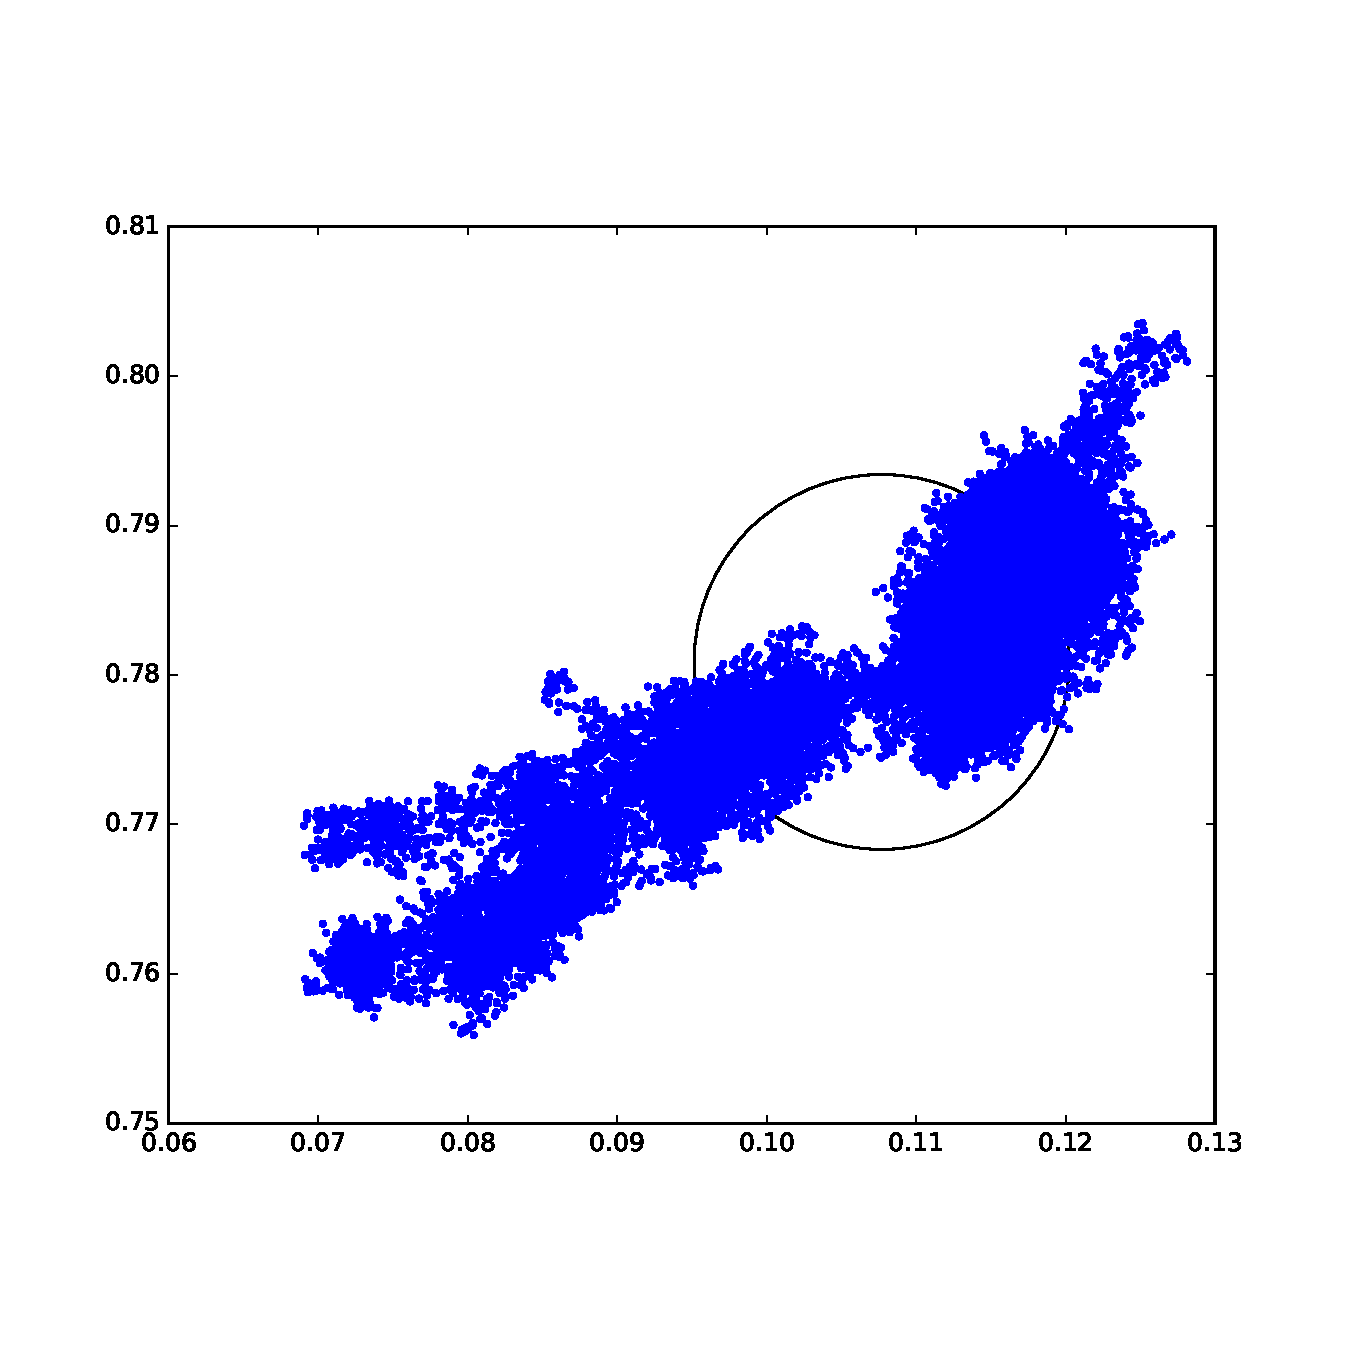
\includegraphics[width=.95\textwidth]{img/03/part_halo_R200.pdf} 
        \caption{La détection des halos par FOF peux être difficile au moment de la reionization car les structure ne sont pas Virialisée
        }
 		\label{fig:part_halo}
\end{figure}

\begin{figure}[bth]
        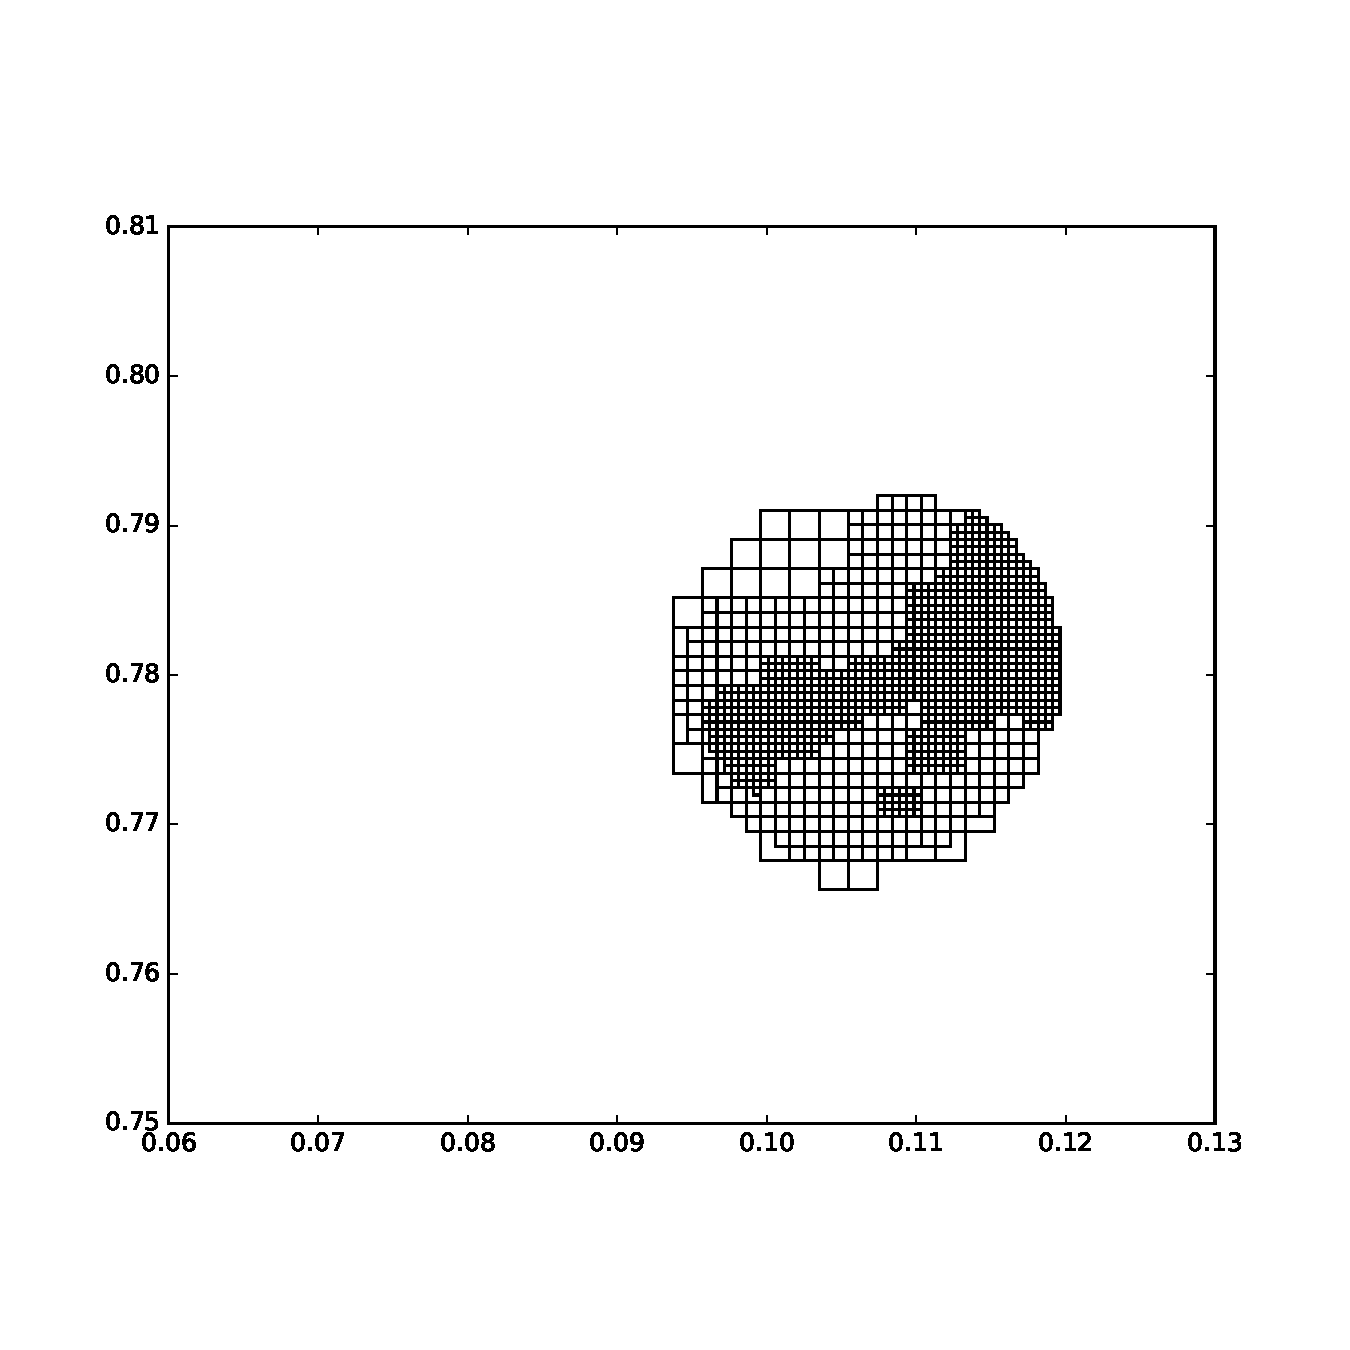
\includegraphics[width=.95\textwidth]{img/03/part_cells.pdf} 
        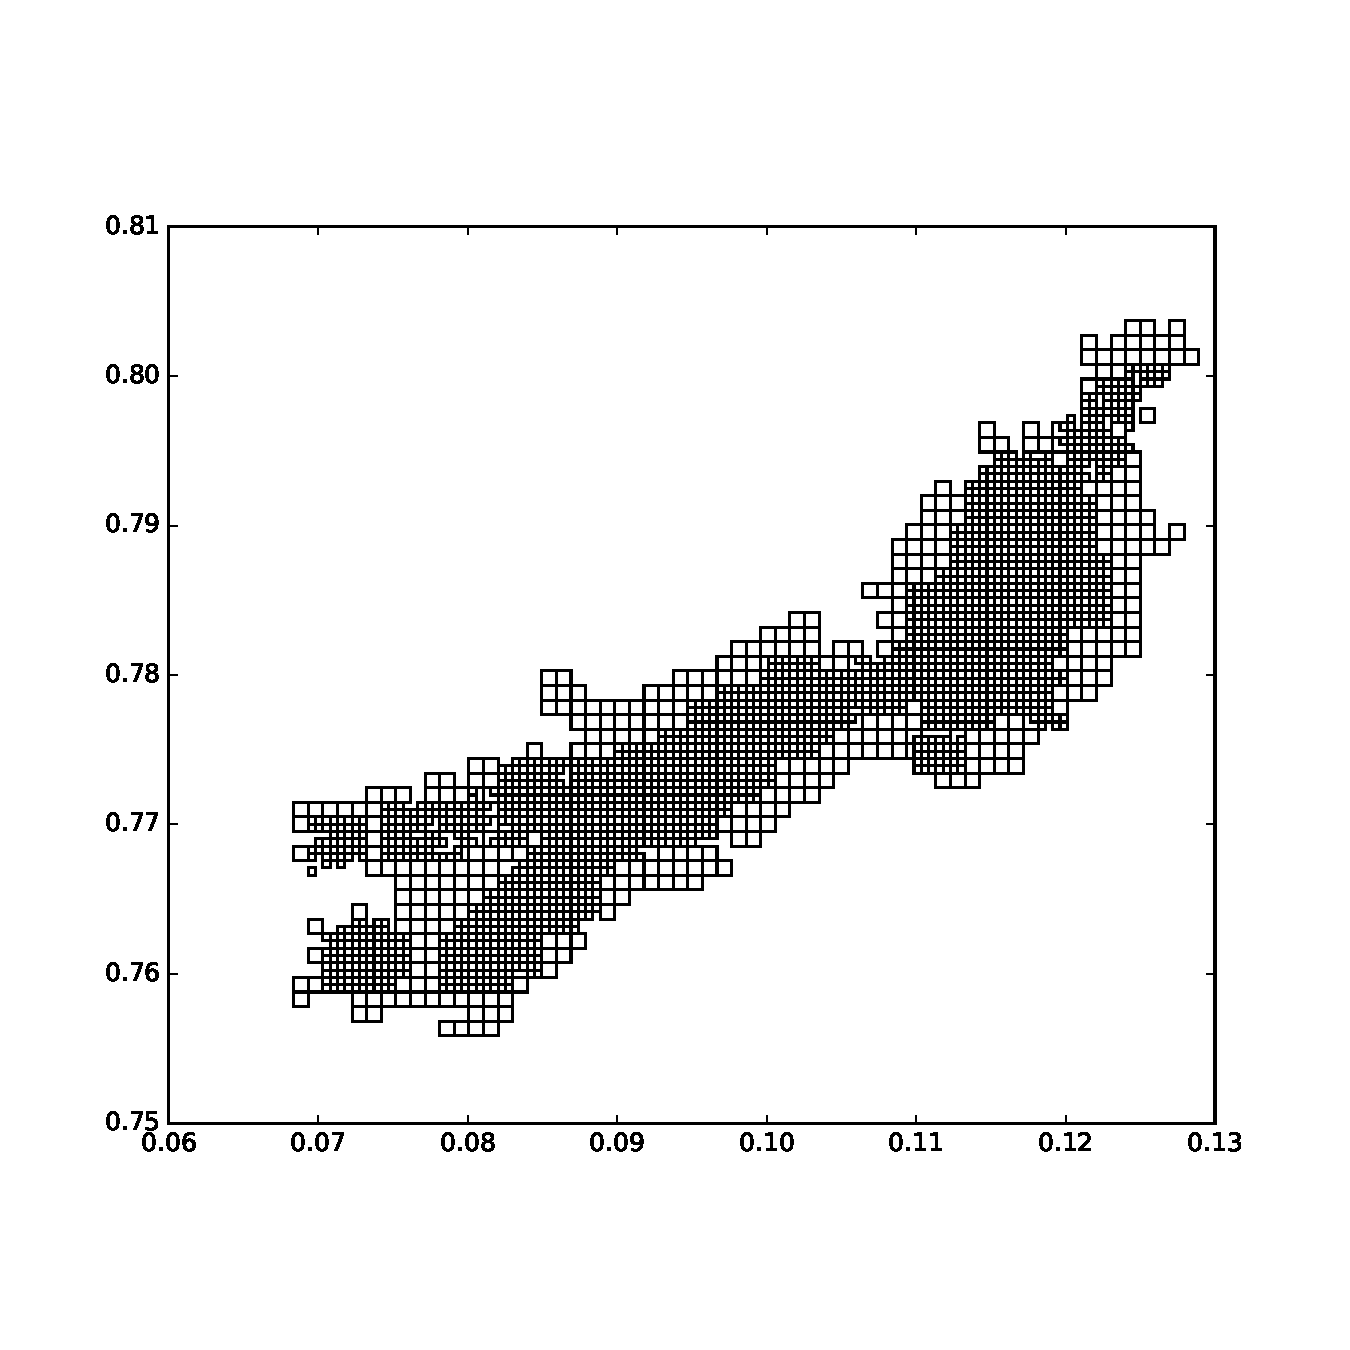
\includegraphics[width=.95\textwidth]{img/03/part_cells_fine.pdf} 
        \caption{La detection des halo par FOF peux être difficile au moment de la reionization car les structure ne sont pas Virialisée
        }
 		\label{fig:part_halo}
\end{figure}




\subsection{association dans le R200}

On cherchera a associer les galaxies  (surdensité d'étoiles) aux halos.
La première méthode consiste a utiliser l'approximation du R200.
Il faudra associer, la matière noire, le gas et les étoiles compris a l'intérieur d'une sphere de rayon R200.

Il sera possible d'utiliser une méthode comparable sur la grille, en utilisant les centres de cellule a la place de la position des étoiles.
Comme les particules de matière noire  données par FoF ne represente pas le meme volume, dans un soucis de cohérence, on appliquera cette méthodes a la matière noire également.

Le méthode est la suivante:

\begin{itemize}
\item générer un KDtree sur les particule de matière noire / les étoiles / la grille AMR
\item Faire une recherche sphérique autour de la positions des halo, sur un rayon de R200
\item stocker les indices dans une structure
\end{itemize}

nous avons donc la possibilité, pour chaque halo, de connaitre n'importe qu'elle grandeur comprisent dans son R200.


Pour les petits halos, peu résolus, la taille des cellules peu être grandes par rapport au R200.
Pour minimiser l'erreur commise, la grille AMR pourra être projeter sur une grille régulière de resolution arbitraire.
Cette méthode permettra d'associer des sous parties de cellules aux halo et améliorera la precision global de l'association.

\subsection{Association "fine"}
Dans le but d'améliorer ces problèmes d'identification dans les halos fortement non virialisé, j'ai développer une méthode pour associer plus précisement les halos et la grille.


la méthode consiste a :
\begin{itemize}
\item générer un KDtree sur la grille
\item pour chaque particule d'une halo, trouver la plus proche cellule
\item filtrer les cellules doublons
\end{itemize}

\section{Étude de la composition dans le R200}


\subsection{La fonction de masse HMF}

\subsection{La masse d'étoiles en fonction de la masse de matière noire + Stellar mass function}
Plus un halo est massif, plus celui ci va contenir d'étoiles.



\subsection{La formation stellaire en fonction de la masse du halo}
Connaissant, a un instant donné, les étoiles appartenant a chaque halo, il est possible de déterminer leurs ages, et donc de connaitre l'histoire de formation stellaire de chaque halo.
Nous allons voir que la masse 

\subsection{La fraction baryonnique}
La fraction baryonique est une grandeur importante pour caractériser un halo.
En effet, le rayonnement n'interagit qu'avec les baryons et plus un halo aura de baryon, plus le rayonnement aura de difficulte a s'en echaper.

\begin{equation}
f_b = \frac{M_* + M_{gas} }{M_{DM} + M_* + M_{gas} }
\end{equation}




\section{Etude au R200}

\subsection{Healpix}
\label{sec:healpix}

Healpix est un outils qui permets de répartir des points de manière uniforme sur la sphere.

\begin{figure}[bth]
        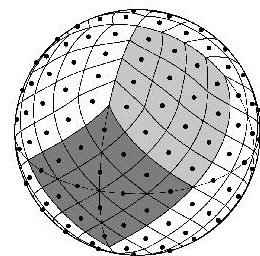
\includegraphics[width=.95\linewidth]{img/03/healpix.jpg} 
        \caption{Exemple de sphere HealPix}
 		\label{fig:HealPix}
\end{figure}

Projection sur la grille AMR
 - utilisation du KD tree
 - nearest neighbhoor
 - récupération des cellules sur la sphere
 

\subsection{Détermination des flux au $R_{200}$}
\label{sec:healpix}

Projection des vecteurs surla normale des cellules de la sphere.

Une question importante dans l’étude de réionisation est la quantité de rayonnement ionisant sortant des halos.
Nous avons vu que le rayonnement interagis les baryons


Pour déterminer les flux autours de chaque halo, il est nécessaire de les englober d'une sphère.
Cette sphère serra discrétisée a l'aide de Healpix (TODO ref) un outils qui permets de répartir des points de manière uniforme sur une surface sphérique (Fig. \ref{fig:HealPix}).
Une fois la sphère générée, on la centrera sur la position du halo, et on la redimensionnera de telle manière a ce qu'elle corresponde aux R200 du halo en question.
Ensuite, pour chaque point de la sphère Healpix, on effectuera une recherche de plus proche voisin, pour déterminer avec qu'elle cellule l'associer.

Nous connaissons maintenant l'ensemble des cellules au R200 de chaques halos.

\subsection{la vitesse du gas au R200}



\subsection{le flux radiatif au R200}
en utilisant cette technique sur 


\section{Influence du feedback stellaire sur la reionization}







\subsection{fraction d'echapement}

%fonction de luminosité 
